\documentclass[12pt,usenames,dvipsnames]{beamer}

%\usetheme[progressbar=frametitle]{metropolis}
\usetheme[subsectionpage=progressbar]{metropolis}

\metroset{block=fill}
%\begin{itemize}[<+- | alert@+>]


\usepackage[utf8]{inputenc}
% Für Häkchen
\usepackage{ pifont }
\newcommand{\cmark}{\ding{51}}%
\newcommand{\xmark}{\ding{55}}%
% Farben
\usepackage{xcolor}

\usepackage{graphicx}
\graphicspath{ {images/} }

\setbeamertemplate{itemize item}{\tiny$\bullet$}
\setbeamertemplate{itemize subitem}{\tiny$\bullet$}

\title{PolyGlot-Database Performance}
\subtitle{Benchmark Framework - MongoDB vs Neo4J}
\author{Hyeon Ung Kim, Tim Niehoff}
%\institute{}
\date{6. August 2018}

\makeatletter
\setbeamertemplate{section page}{
  \centering
  \begin{minipage}{22em}
    \raggedright
    \usebeamercolor[fg]{section title}
    \usebeamerfont{section title}
    \centering\insertsectionhead\\[-1ex]
    \centering\usebeamertemplate*{progress bar in section page}
    \par
    \ifx\insertsubsectionhead\@empty\else%
      \usebeamercolor[fg]{subsection title}%
      \usebeamerfont{subsection title}%
      \centering\insertsubsectionhead
    \fi
  \end{minipage}
  \par
  \vspace{\baselineskip}
}
\makeatother

\begin{document}

	\maketitle
			
%	\begin{frame}{Gliederung}
%		\setbeamertemplate{section in toc}[sections numbered]
%\setbeamertemplate{subsection in toc}[subsections numbered]
%		\tableofcontents
%	\end{frame}
	\section{Aufgabenstellung}
	\begin{frame}{Heranführung}
	\begin{itemize}[<+- | alert@+>]
	\item Verschiedene DB Typen mit unterschiedlichen Vorteilen\footnote{ Inhalt der Folie von \url{https://dbs.uni-leipzig.de/file/Intro_bdprak_final.pdf}}
		\begin{itemize} [<+- | alert@+>]
	\item Relational: Sicherheit, homogene Daten
	\item Document: Flexibles Schema, Suchfunktionen
	\item Graph: Beziehungen, Traversal
	\end{itemize}
	\item Polyglot: Verwendung mehrerer DB-Typen für untersch. Anwendungsfälle
	\item Aufgabe: Vergleich einer
Graphdatenbank mit einer Dokumenten-Datenbank
	\end{itemize}	
	\end{frame}
		\begin{frame}{gegebene Werkzeuge}
		\begin{table}[]
\begin{tabular}{ll}

\includegraphics[width=0.2\textwidth]{java}  & 
\includegraphics[width=0.3\textwidth]{yelp} \\

\includegraphics[width=0.4\textwidth]{mongodb}  & 
\includegraphics[width=0.35\textwidth]{neo4j}
\end{tabular}
\end{table}
	\end{frame}
\begin{frame}<presentation:0>
\begin{itemize}
\item Mongo + Neo4j Driver
\item teilweise nicht ausgereift. Für das garantieren von beliebigen Queries muss geparst werden
\end{itemize}
\end{frame}
\section{Herausforderung: Gleicher Datensatz auf beiden DB}
\subsection{Mongo Connector + Neo4j Doc Manager}
\begin{frame}{Mongo Connector + Neo4j Doc Manager}
\begin{itemize}[<+- | alert@+>]
\item Software jeweils von MongoDB und Neo4j
\item Dauerhafte Synchronisation zwischen Mongo und Neo4j möglich
\item Generisches Erstellen des Neo4j Datenmodells 
\end{itemize}
\end{frame}
\subsection{Apoc}
\begin{frame}
\begin{itemize}[<+- | alert@+>]
\item Software von Neo4j zum Import von JSONs in Neo4j
\item keine automatische Synchronisierung zwischen Mongo und Neo4j
\item kein generisches Datenmodell
\item Vorteil des nutzerspezifischen Datenmodells: Ausnutzen graphdatenbankspezifischer Performanzvorteile
\end{itemize}

\end{frame}
\section{Resultat: PolyGDBP}
\subsection{Features}
\begin{frame}
\begin{itemize}[<+- | alert@+>]
\item Command line Interface mit Parametereingabe (Query, Serveradressen, Datensatz, ...)
\item Obligatorisch nur Queryangabe 
\item Vorgefertigte Queries für Yelp Datensatz, ansonsten Angabe benutzerspezifischer Queries
\item Reduzieren und Einlesen des Datensatzes möglich (via MongoAPI und MongoConnector)
\item Vor und nach jedem Schritt Stoppen der Zeit, Logging, Filewriting
\item Visualisierung mittels Javascript Anwendung möglich
\end{itemize}
\end{frame}
\begin{frame}{Programmstruktur}
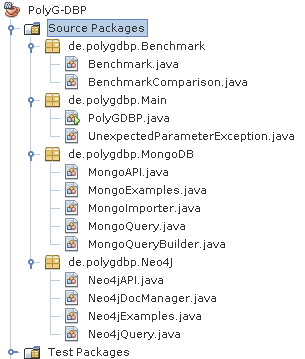
\includegraphics[width=0.6\textwidth]{files}

\end{frame}
\section{Tests mit dem Yelp Dataset}
\subsection{Datensatz + DatenModell}
\begin{frame}
\begin{itemize}[<+- | alert@+>]
\item Yelp = Suchmaschine und Empfehlungsportal für Restaurants und Geschäfte 
\item Datensatz $\geq$ 6,5 GB
\item besteht aus 6 *.jsons: business, checkin, photos, review, tip,  user
\item 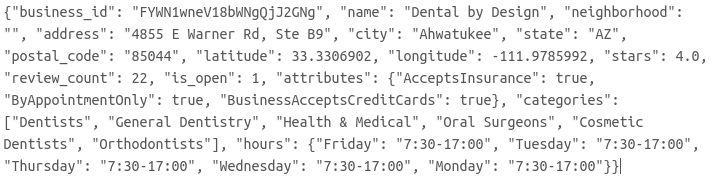
\includegraphics[width=1.0\textwidth]{business}
\end{itemize}
\end{frame}
\begin{frame}{Neo4j Datenmodell}
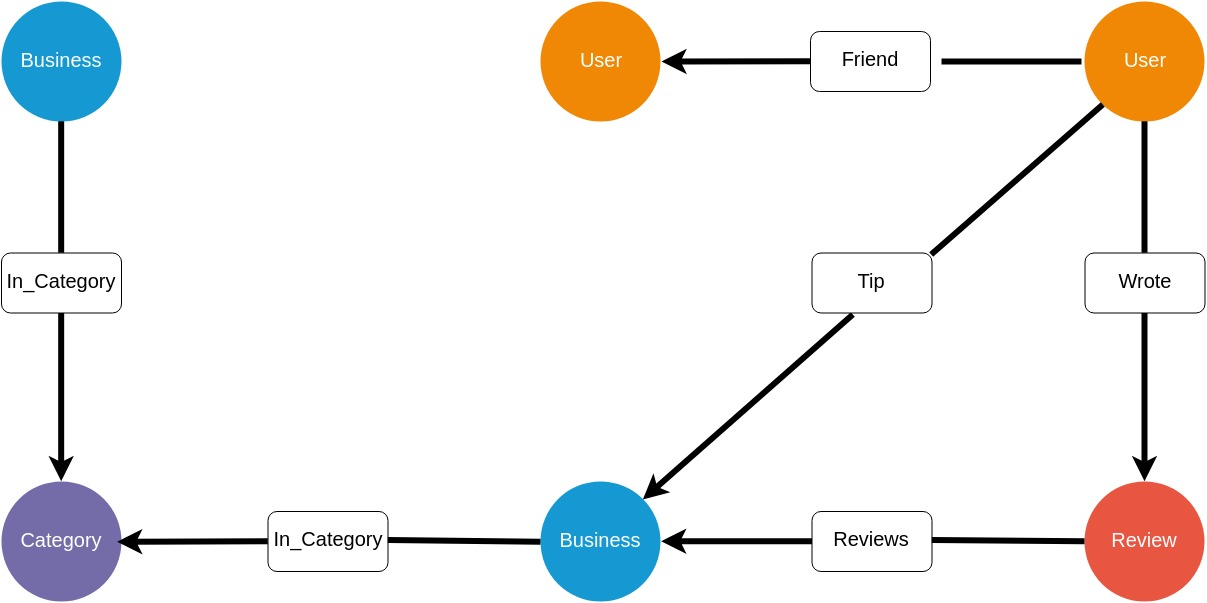
\includegraphics[width=1\textwidth]{neo4jModell}

\end{frame}
\subsection{Ergebnisse}
	\section{Zusammenfassung}
	\begin{frame}{Zusammenfassung}
	\begin{itemize}[<+- | alert@+>]
	\item Verschiedene DB-Typen mit versch. Vor- und Nachteile
	\item PolyG-DBP = Framework zum Vergleich einer Dokument-DB mit einer Graphdatenbank
	\item konkret: MongoDB und Neo4j werden getestet
	\item Ausführung von prebuilt Queries oder nutzerspezifischen Queries
	\item Messen und Vergleich der Query-Ausführungszeiten
	\item Vergleich Neo4j und MongoDB mit Yelp Datensatz: MongoDB performanter bei einfachen Queries, Neo4j siegt bei Queries mit mehreren Relationen/Collections
	\end{itemize}
	\end{frame}
\begin{frame}[standout]
  Fragen und Diskussion
\end{frame}


\end{document}